\documentclass[10pt,a4paper]{report}
\usepackage[utf8]{inputenc}
\usepackage{amsmath}
\usepackage{amsfonts}
\usepackage{amssymb}
\usepackage{amsthm}
\usepackage{hyperref}

\usepackage{multicol}
\usepackage{fancyhdr}
\usepackage[inline]{enumitem}
\usepackage{tikz}
\usepackage{tikz-cd}
\usetikzlibrary{calc}
\usetikzlibrary{shapes.geometric}
\usetikzlibrary{positioning}
\usepackage[margin=0.5in]{geometry}
\usepackage{xcolor}

\hypersetup{
    colorlinks=true,
    linkcolor=blue,
    filecolor=magenta,      
    urlcolor=cyan,
    pdftitle={Tensors},
    pdfpagemode=FullScreen,
    }

%\urlstyle{same}

\newcommand{\CLASSNAME}{Math 5050 -- Special Topics: Manifolds}
\newcommand{\STUDENTNAME}{Paul Carmody}
\newcommand{\ASSIGNMENT}{Section 7: Quotients }
\newcommand{\DUEDATE}{May 17, 2025}
\newcommand{\PROFESSOR}{Professor Berchenko-Kogan}
\newcommand{\SEMESTER}{Fall 2025}
\newcommand{\SCHEDULE}{TBD}
\newcommand{\ROOM}{Remote}

\newcommand{\MMN}{M_{m\times n}}
\newcommand{\FF}{\mathcal{F}}

\pagestyle{fancy}
\fancyhf{}
\chead{ \fancyplain{}{\CLASSNAME} }
%\chead{ \fancyplain{}{\STUDENTNAME} }
\rhead{\thepage}
\newcommand{\LET}{\text{Let }}
%\newcommand{\IF}{\text{if }}
\newcommand{\AND}{\text{ and }}
\newcommand{\OR}{\text{ or }}
\newcommand{\FORSOME}{\text{ for some }}
\newcommand{\FORALL}{\text{ for all }}
\newcommand{\WHERE}{\text{ where }}
\newcommand{\WTS}{\text{ WTS }}
\newcommand{\WLOG}{\text{ WLOG }}
\newcommand{\BS}{\backslash}
\newcommand{\DEFINE}[1]{\textbf{\emph{#1}}}
\newcommand{\IF}{$(\Rightarrow)$}
\newcommand{\ONLYIF}{$(\Leftarrow)$}
\newcommand{\ITH}{\textsuperscript{th} }
\newcommand{\FST}{\textsuperscript{st} }
\newcommand{\SND}{\textsuperscript{nd} }
\newcommand{\TRD}{\textsuperscript{rd} }
\newcommand{\INV}{\textsuperscript{-1} }


%%%%%%%
% derivatives
%%%%%%%

\newcommand{\PART}[2]{\frac{\partial #1}{\partial #2}}
\newcommand{\SPART}[2]{\frac{\partial^2 #1}{\partial #2^2}}
\newcommand{\DERIV}[2]{\frac{d #1}{d #2}}
\newcommand{\LAPLACIAN}[1]{\frac{\partial^2 #1}{\partial x^2} + \frac{\partial^2 #1}{\partial y^2}}

%%%%%%%
% sum, product, union, intersections
%%%%%%%

\newcommand{\SUM}[2]{\underset{#1}{\overset{#2}{\sum}}}
\newcommand{\PROD}[2]{\underset{#1}{\overset{#2}{\prod}}}
\newcommand{\UNION}[2]{\underset{#1}{\overset{#2}{\bigcup}}}
\newcommand{\INTERSECT}[2]{\underset{#1}{\overset{#2}{\bigcap}}}
\newcommand{\FSUM}{\SUM{n=-\infty}{\infty}}
       

%%%%%%%
% supremum and infimum
%%%%%%%

\newcommand{\SUP}[1]{\underset{#1}\sup \,}
\newcommand{\INF}[1]{\underset{#1}\inf \,}
\newcommand{\MAX}[1]{\underset{#1}\max \,}
\newcommand{\MIN}[1]{\underset{#1}\min \,}

%%%%%%%
% infinite sums, limits
%%%%%%%

\newcommand{\SUMK}{\SUM{k=1}{\infty}}
\newcommand{\SUMN}{\SUM{n=1}{\infty}}
\newcommand{\SUMKZ}{\SUM{k=0}{\infty}}
\newcommand{\LIM}[1]{\underset{#1}\lim\,}
\newcommand{\IWOB}[1]{\LIM{#1 \to \infty}}
\newcommand{\LIMK}{\IWOB{k}}
\newcommand{\LIMN}{\IWOB{n}}
\newcommand{\LIMX}{\IWOB{x}}
\newcommand{\NIWOB}{\LIM{n \to \infty}}
\newcommand{\LIMSUPK}{\underset{k\to\infty}\limsup \,}
\newcommand{\LIMSUPN}{\underset{n\to\infty}\limsup \,}
\newcommand{\LIMINFK}{\underset{k\to\infty}\liminf \,}
\newcommand{\LIMINFN}{\underset{n\to\infty}\liminf \,}
\newcommand{\ROOTRULE}[1]{\LIMSUPK \BARS{#1}^{1/k}}

\newcommand{\CUPK}{\bigcup_{k=1}^{\infty}}
\newcommand{\CAPK}{\bigcap_{k=1}^{\infty}}
\newcommand{\CUPN}{\bigcup_{n=1}^{\infty}}
\newcommand{\CAPN}{\bigcap_{n=1}^{\infty}}

%%%%%%%
% number systems (real, rational, etc.)
%%%%%%%

\newcommand{\REALS}{\mathbb{R}}
\newcommand{\RATIONALS}{\mathbb{Q}}
\newcommand{\IRRATIONALS}{\REALS \backslash \RATIONALS}
\newcommand{\INTEGERS}{\mathbb{Z}}
\newcommand{\NUMBERS}{\mathbb{N}}
\newcommand{\COMPLEX}{\mathbb{C}}
\newcommand{\DISC}{\mathbb{D}}
\newcommand{\HPLANE}{\mathbb{H}}

\newcommand{\R}{\mathbb{R}}
\newcommand{\Q}{\mathbb{Q}}
\newcommand{\Z}{\mathbb{Z}}
\newcommand{\N}{\mathbb{N}}
\newcommand{\C}{\mathbb{C}}
\newcommand{\T}{\mathbb{T}}
\newcommand{\COUNTABLE}{\aleph_0}
\newcommand{\UNCOUNTABLE}{\aleph_1}


%%%%%%%
% Arithmetic/Algebraic operators
%%%%%%%


\DeclareMathOperator{\MOD}{mod}
%\newcommand{\MOD}[1]{\mod #1}
\newcommand{\BAR}[1]{\overline{#1}}
\newcommand{\LCM}{\text{ lcm}}
\newcommand{\ZMOD}[1]{\Z/#1\Z}
\DeclareMathOperator{\VAR}{Var}
%%%%%%%
% complex operators
%%%%%%%

\DeclareMathOperator{\RR}{Re}
%\newcommand{\RE}{\text{Re}}
\DeclareMathOperator{\IM}{Im}
%\newcommand{\IM}{\text{Im}}
\newcommand{\CONJ}[1]{\overline{#1}}
\DeclareMathOperator{\LOG}{Log}
%\newcommand{\LOG}{\text{ Log }}
\newcommand{\RES}[2]{\underset{#1}{\text{res}} #2}

%%%%%%%
% Group operators
%%%%%%%

\newcommand{\AUT}{\text{Aut}\,}
\newcommand{\KER}{\text{ker}\,}
\newcommand{\END}{\text{End}}
\newcommand{\HOM}{\text{Hom}}
\newcommand{\CYCLE}[1]{(\begin{array}{cccccccccc}
		#1
	\end{array})}
\newcommand{\SUBGROUP}{\underset{\text{group}}\subseteq}	
%\newcommand{\SUBGROUP}{\subseteq_g}
\newcommand{\SUBRING}{\underset{\text{ring}}\subseteq}
\newcommand{\SUBMOD}{\underset{\text{mod}}\subseteq}
\newcommand{\SUBFIELD}{\underset{\text{field}}\subseteq}
\newcommand{\ISO}{\underset{\text{iso}}\longrightarrow}
\newcommand{\HOMO}{\underset{\text{homo}}\longrightarrow}

%%%%%%%
% grouping (parenthesis, absolute value, square, multi-level brackets).
%%%%%%%

\newcommand{\PAREN}[1]{\left (\, #1 \,\right )}
\newcommand{\BRACKET}[1]{\left \{\, #1 \,\right \}}
\newcommand{\SQBRACKET}[1]{\left [\, #1 \,\right ]}
\newcommand{\ABRACKET}[1]{\left \langle\, #1 \,\right \rangle}
\newcommand{\BARS}[1]{\left |\, #1 \,\right |}
\newcommand{\DBARS}[1]{\left \| \, #1 \,\right \|}
\newcommand{\LBRACKET}[1]{\left \{ #1 \right .} 
\newcommand{\RBRACKET}[1]{\left . #1 \right \]}
\newcommand{\RBAR}[1]{\left . #1 \, \right |}
\newcommand{\LBAR}[1]{\left | \, #1 \right .}
\newcommand{\BLBRACKET}[2]{\BRACKET{\RBAR{#1}#2}}
\newcommand{\GEN}[1]{\ABRACKET{#1}}
\newcommand{\BINDEF}[2]{\LBRACKET{\begin{array}{ll}
     #1\\
     #2
\end{array}}}

%%%%%%%
% Fourier Analysis
%%%%%%%

\newcommand{\ONEOTWOPI}{\frac{1}{2\pi}}
\newcommand{\FHAT}{\hat{f}(n)}
\newcommand{\FINT}{\int_{-\pi}^\pi}
\newcommand{\FINTWO}{\int_{0}^{2\pi}}
\newcommand{\FSUMN}[1]{\SUM{n=-#1}{#1}}
%\newcommand{\FSUM}{\SUMN{\infty}}
\newcommand{\EIN}[1]{e^{in#1}}
\newcommand{\NEIN}[1]{e^{-in#1}}
\newcommand{\INTALL}{\int_{-\infty}^{\infty}}
\newcommand{\FTINT}[1]{\INTALL #1 e^{2\pi inx\xi} dx}
\newcommand{\GAUSS}{e^{-\pi x^2}}

%%%%%%%
% formatting 
%%%%%%%

\newcommand{\LEFTBOLD}[1]{\noindent\textbf{#1}}
\newcommand{\SEQ}[1]{\{#1\,\}}
\newcommand{\WIP}{\footnote{work in progress}}
\newcommand{\QED}{\hfill\square}
\newcommand{\ts}{\textsuperscript}
\newcommand{\HLINE}{\noindent\rule{7in}{1pt}\\}

%%%%%%%
% Mathematical note taking (definitions, theorems, etc.)
%%%%%%%

\newcommand{\REM}{\noindent\textbf{\\Remark: }}
\newcommand{\DEF}{\noindent\textbf{\\Definition: }}
\newcommand{\THE}{\noindent\textbf{\\Theorem: }}
\newcommand{\COR}{\noindent\textbf{\\Corollary: }}
\newcommand{\LEM}{\noindent\textbf{\\Lemma: }}
\newcommand{\PROP}{\noindent\textbf{\\Proposition: }}
\newcommand{\PROOF}{\noindent\textbf{\\Proof: }}
\newcommand{\EXP}{\noindent\textbf{\\Example: }}
\newcommand{\TRICKS}{\noindent\textbf{\\Tricks: }}


%%%%%%%
% text highlighting
%%%%%%%

\newcommand{\B}[1]{\textbf{#1}}
\newcommand{\CAL}[1]{\mathcal{#1}}
\newcommand{\UL}[1]{\underline{#1}}

%%%%%%
% Linear Algebra
%%%%%%

\newcommand{\COLVECTOR}[1]{\PAREN{\begin{array}{c}
#1
\end{array} }}
\newcommand{\TWOXTWO}[4]{\PAREN{ \begin{array}{c c} #1&#2 \\ #3 & #4 \end{array} }}
\newcommand{\THREEXTHREE}[9]{\PAREN{ \begin{array}{c c c} #1&#2&#3 \\ #4 & #5 & #6 \\ #7 & #8 & #9 \end{array} }}
\newcommand{\NXN}{\PAREN{ \begin{array}{c c c c} 
			a_{11} & a_{12} & \cdots & a_{1n} \\
			a_{21} & a_{22} & \cdots & a_{2n} \\
			\vdots & \vdots & \ddots & a_{1n} \\
			a_{n1} & a_{n2} & \cdots & a_{nn} \\
		\end{array} }}
\newcommand{\SLR}{SL_2(\R)}
\newcommand{\GLR}{GL_2(\R)}
\DeclareMathOperator{\TR}{tr}
\DeclareMathOperator{\BIL}{Bil}
\DeclareMathOperator{\SPAN}{span}

%%%%%%%
%  White space
%%%%%%%

\newcommand{\BOXIT}[1]{\noindent\fbox{\parbox{\textwidth}{#1}}}


\newtheorem{theorem}{Theorem}[section]
\newtheorem{corollary}{Corollary}[theorem]
\newtheorem{lemma}[theorem]{Lemma}

\theoremstyle{definition}
\newtheorem{definition}[theorem]{Definition}
\newtheorem{prop}[theorem]{Proposition}

\theoremstyle{remark}
\newtheorem{remark}[theorem]{Remark}
\newtheorem{example}[theorem]{Example}
%\newtheorem*{proof}[theorem]{Proof}



\newcommand{\RED}[1]{\textcolor{red}{#1}}
\newcommand{\BLUE}[1]{\textcolor{blue}{#1}}

\begin{document}

\begin{center}
	\Large{\CLASSNAME -- \SEMESTER} \\
	\large{ w/\PROFESSOR}
\end{center}
\begin{center}
	\STUDENTNAME \\
	\ASSIGNMENT -- \DUEDATE\\
\end{center} 

\noindent\textbf{Pg. 77: Exercise 7.11 (Real projective space as a quotient of a sphere).*}  For $x=(x^1,\dots,x^n)\in \R^n$, let $||x|| = \sqrt{\sum_i(x^i)^2}$ be the modulus of $x$.  Prove that the map $f: \R^{n+1} - \{0\} \to S^n$ given by 
\begin{align*}
	f(x) = \frac{x}{||x||}
\end{align*}induces a homeomorphism $\bar{f}: \R P^n\to S^n/\sim$.  Where
\begin{align*}
	x \sim y &\iff x=\pm y, \, x,y \in S^n
\end{align*} (\textit{Hint: } Find an inverse map 
\begin{align*}
	\bar{g}: S^n/\sim \,\to \R P^n
\end{align*}and show that both $\bar{f}$ and $\bar{g}$ are continuous.)\\

\BLUE{Given the relation above $x \sim y \iff x=\pm y,\, x,y \in S^n$.  Define
	\begin{align*}
		\bar{g}([x]) &= [x] 
	\end{align*}Note that on the left $[x] \in S^n/\sim$ and $[x] \in \R P^n$.  For clarity,\footnote{$\R P^n \equiv \R^{n+1}/r(x,y)$ where $r(x,y)$ is the relation that is true when $x,y,p$ are colinear.} 
	\begin{align*}
		[a] \in S^n/\sim &\implies [a] = \{ a, -a\} \WHERE a \in S^n\\
		[b] \in \R P^n &\implies [b] = \{x \in \R^{n+1}|\, x=\alpha b,\, \forall \alpha \in \R\} \WHERE b \in \R^{n+1} 
	\end{align*}Notice that
	\begin{align*}
		\bar{f}([b]) &= [f(b)] = \SQBRACKET{\frac{b}{||b||}} \in S^n/\sim \\
		\bar{g}\PAREN{\SQBRACKET{\frac{b}{||b||}}} &= [b] \\
		\therefore \bar{g}\circ\bar{f} = \mathbb{I}\\
		\AND \bar{g}([a]) &= [a] \in \R P^n \\
		\bar{f}\PAREN{\bar{g}([a])} &= \SQBRACKET{\frac{[a]}{|| [a]||}} = [f(a)] = [a] \in S^n/\sim\\
		\therefore \bar{f}\circ\bar{g} = \mathbb{I}
	\end{align*} $\bar{f}$ is continuous because $f$ is continuous.  $\bar{g}$ is continuous because it is a mapping of one identity to another.  Therefore, $\bar{f}$ is a homeomorphism.
	}
	
\HLINE
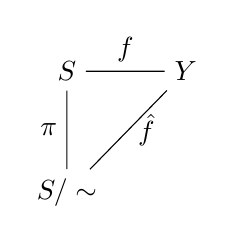
\begin{tikzpicture}
	\node (S) {$S$};
	\node (Y)  [right=of S] {$Y$};
	\node (Q)  [below= of S] {$S/\sim$};
	\draw (S) -> node[above] {$f$} (Y) 
		(S) ->  node[left] {$\pi$} (Q)
		(Q) -> node[right] {$\hat{f}$} (Y);
\end{tikzpicture}\\
\textbf{Problems}

\begin{enumerate}[label=7.\arabic*.]
	\item \textbf{Image of the inverse image of a map}
	
	Let $f:X\to Y$ be a map of sets, and let $B \subset Y$.  Prove that $f(f^{-1}(B)) = B \cap f(X)$.  Therefore, if $f$ is surjective, then $f(f^{-1}(B)) = B$.
	
	\BLUE{\textbf{$\subseteq$:  }Let $b \in B$ and $a \in X$ such that $f(a) = b$.  Then, $a \in f^{-1}(b)$, thus $a$ is an arbitrary point in $f^{-1}(B)$.  We know that $f(a) \in f(X)$ and $f(a) \in B$, therefore $f(a) \in B \cap f(X)$ and $f(f^{-1}(B)) \subseteq B \cap f(X)$.\\ \\
	\textbf{$\supseteq$:  }Let $b \in B \cap  f(X)$.  Since $b \in f(X)$, there exists $a \in X$ such that $f(a) = b$ and since $b \in B$ then $b = f(a) \in f(f^{-1}(b)) \subseteq f^{-1}(B)$.  Therefore $b \in f(f^{-1}(B))$\\
	}
	
	\item \textbf{Real projective plane}
	
	Let $H^2$ be the closed upper hemisphere in the unit sphere $S^2$, and let $i: H^2 \to S^2$ be the inclusion map.  In the notation of example 7.13, prove that the induced map $f: H^2/\sim \,\to S^2/\sim$ is a homeomorphism. (\textit{Hint:} Imitate Propostion 7.3.)
\newcommand{\HOMEO}{\overset{\sim}\to}	
	\BLUE{Let $H^2$ be the upper hemisphere and $S^2$ be the unit sphere
	\begin{align*}
		H^2 &= \{(x,y,z) \in \R^3\,|\, x^2+y^2+z^2=1, z \ge 0\} \\
		S^2 &= \{(x,y,z) \in \R^3\,|\, x^2+y^2+z^2=1\}
	\end{align*}These two are homeomorphic to each via 
	\begin{align*}
		\varphi : S^2 &\mapsto H^2 \\
		\varphi(x,y,z) &= (x,y, |z|)
	\end{align*} and its inverse
	\begin{align*}
		\psi : H^2 &\mapsto S^2 \\
		\psi(x,y,z) &= (x,y,z)
	\end{align*}Define the relations
	\begin{align*}
		(x,y,z) \sim (-x,-y,-z) &\to x^2+y^2=z^2, \, \forall (x,y,z) \in S^2 \\
		(x,y,z) \sim (x,y, z) &\to \sqrt{x^2+y^2}=z, \, \forall (x,y,z) \in H^2
	\end{align*}Then we induce $f:H^2/\sim\, \to S^2/\sim$ as
	\begin{align*}
		f([(x,y,z)]) &= [(x,y,z)]
	\end{align*}
	}
	
	\item \textbf{Closedness of the diagonal of a Hausdorff Space}
	
	Deduce Theorem 7.7 from Corollary 7.8 (\textit{Hint:} To prove that if $S/\sim$ is Hausdorff, then the graph $R$ of $\sim$ is closed in $S \times S$, use the continuity of the projection map $\pi:S \to S/\sim$.  To prove the reverse implication, use the openness of $\pi$.)
	
	\item \textbf{Quotient of a sphere with antipodal points indentified}
	
	Let $S^n$ be the unit sphere centered at the oringin $\R^{n+1}$.  Define an equivalence relation $\sim$ on $S^n$ by indentifying antipodal points:
	\begin{align*}
		x \sim y \iff x=\pm y, \, x,y, \in S^n
	\end{align*}\begin{enumerate}[label=(\alph*)]
		\item Show that $\sim$ is an open equivalence relation.
		\item Apply Theorem 7.7 and Corallary 7.8 to prove that the quotient space $S^n/\sim$ is Hausdorff, without making use of the homeomorphism $\R P^n \cong S^n/\sim$.
	\end{enumerate}
	
	\item \textbf{Orbit space of a continuous group action}
	
	Suppose a right action of a topological group $G$ on a topological space $S$ is continuous, this simply imeans that the map $S \times G \to S$ describing teh action is continuous.  Define two points $x,y$ of $S$ to bequivalent if they are in teh same orbit; i.e., there is an element $g \in G$ such that $y=xg$.  Let $S/G$ be teh quotient space; it is called the \textit{orbit space} of the action.  Prove that the projection map $\pi: S \to S/G$ is an open map.  (This problem generlaizes Proposition 7.14, in which $G=R^\times = \R-\{0\}$ and $S = \R^{n+1}-\{0\}$.  Because $\R^\times$ is commutative, a left $\R^\times$-action becomes a right $\R^\times$-action if scalar multiplicatin is written on teh right.)
	
	\item \textbf{Quotient of $\R$ by $2\pi\Z$.}
	
	Let the addtivei group $2\Z$ act on $\R$ on the right by $x\cdot 2\pi n=x+2\pi n$, where $n$ is an integer.  Show that eh orbit space $\R/2\pi\Z$ is a smooth manifold.
	
	\item \textbf{The circle asa quotient space}
	
	\begin{enumerate}[label=(\alph*)]
	
		\item Let $\{(U_\alpha, \phi_\alpha)\{_{\alpha=1}^2$ be the atlas of circles $S^1$ in Example 5.7, and let $\bar{\phi}_\alpha$ be the map $\phi_\alpha$ followed by the projection $\R \to \R/2\pi\Z$.  On $U_1\cap U_2 = A \coprod B$, since $\phi_1$ and $\phi_2$ differ by an integer multiple of $2\pi$, $\bar{\phi}_1 = \bar{phi}_2$.  Therefore, $\bar{\phi}_1$ and $\bar{\phi}_2$ piece together to give a well-defined map $\bar{\phi}: S^1\to \R/2\pi\Z$.  Prove that $\bar{\phi}$ is $C^\infty$.
		
		\item The complex exponetial $\R \to S^1, t\mapsto e^{it}$, is constant on each orbit of the action of $2\pi\Z$ on $\R$.  Therefore, there is an induced map $F: \R/2\pi\Z \to S^1, F([t])=e^{it}$.  Prove that $F$ is $C^\infty$.
		
		\item Prove that $F: \R/2\pi/Z \to S^1$ is a diffeomorphism.
	
	\end{enumerate}
	
	\item \textbf{The Grassmanian $G(k,n)$}
	
	\item \textbf{Compactness of real projective space}
	
	Show that the real projective space $\R P^n$ is compact. (\textit{Hint:} Use Exercise 7.11.)
	

\end{enumerate}
\end{document}
